\documentclass[10pt, compress]{beamer}

\usetheme{m}

\usepackage{booktabs}
\usepackage[scale=2]{ccicons}
\usepackage{minted}
\usepackage{hyperref}
\usepackage{multicol,graphicx}
\usepackage{gb4e}
\resetcounteronoverlays{exx}

\usemintedstyle{trac}

\title{Tackling Natural Language Generation Challenges at Narrative Science}
\subtitle{}
\date{Oct 19, 2017}
\author{Mike Pham \& Clayton Norris}
\institute{Narrative Science}

\begin{document}

\maketitle

% Company Overview
% Platform overview
% [Transition into main topic]
%   Machine learning is not a feature
% Deep dive on problems:
%   Verb conjugation
%       Can you machine learn verb forms? Talk to John Goldsmith
%       Rule based approaches kind of work, but you keep having to add exceptions for irregular verbs
%           This varies language to language
%       Really it’s not that hard to just enumerate all verbs with their forms, there aren’t that many verbs that people use
%   Pronouns
%       Take a passage of text with all specific references, ask audience: how do we get it to be less redundant?
%           Maybe use a real passage and replace refs with specific?
%       Go through some rule-based approaches, show where that either gets hairy or doesn’t work
%       “This is a well studied phenomenon called saliency”
%   Sentence selection
%       You obviously can’t enumerate all good sentences
%       Rule systems are just really inextensible
%       This is really hard to pin down, finally a good problem to apply machine learning to
% Conclusions
% Talk about internships now or at the beginning?
% Q&A

\section{Overview}
\begin{frame}{What is Quill?}
    Quill is an \alert{Advanced Natural Language Generation (NLG)} platform

    \begin{description}
        \item[NLG] A form of artificial intelligence (AI) that automatically produces language from structured data. 
        \item[intent-driven] Advanced NLG uses \alert{intent}, or what you want to know, as its guide from the very beginning.
    \end{description}
\end{frame}

\begin{frame}{How is this different than other NLG?}
	So what?
	\pause

	\begin{itemize}
		\item How is this different than Amazon sending me a templated email receipt of my recent purchases?	\pause
		\item What about all those neural nets generating facebook posts that sound eeriely like my previous posts?	\pause
	\end{itemize}
\end{frame}

\begin{frame}{Other NLG}
	\alert{trigger warning: offensive language}
	\pause
	\begin{multicols}{2}
		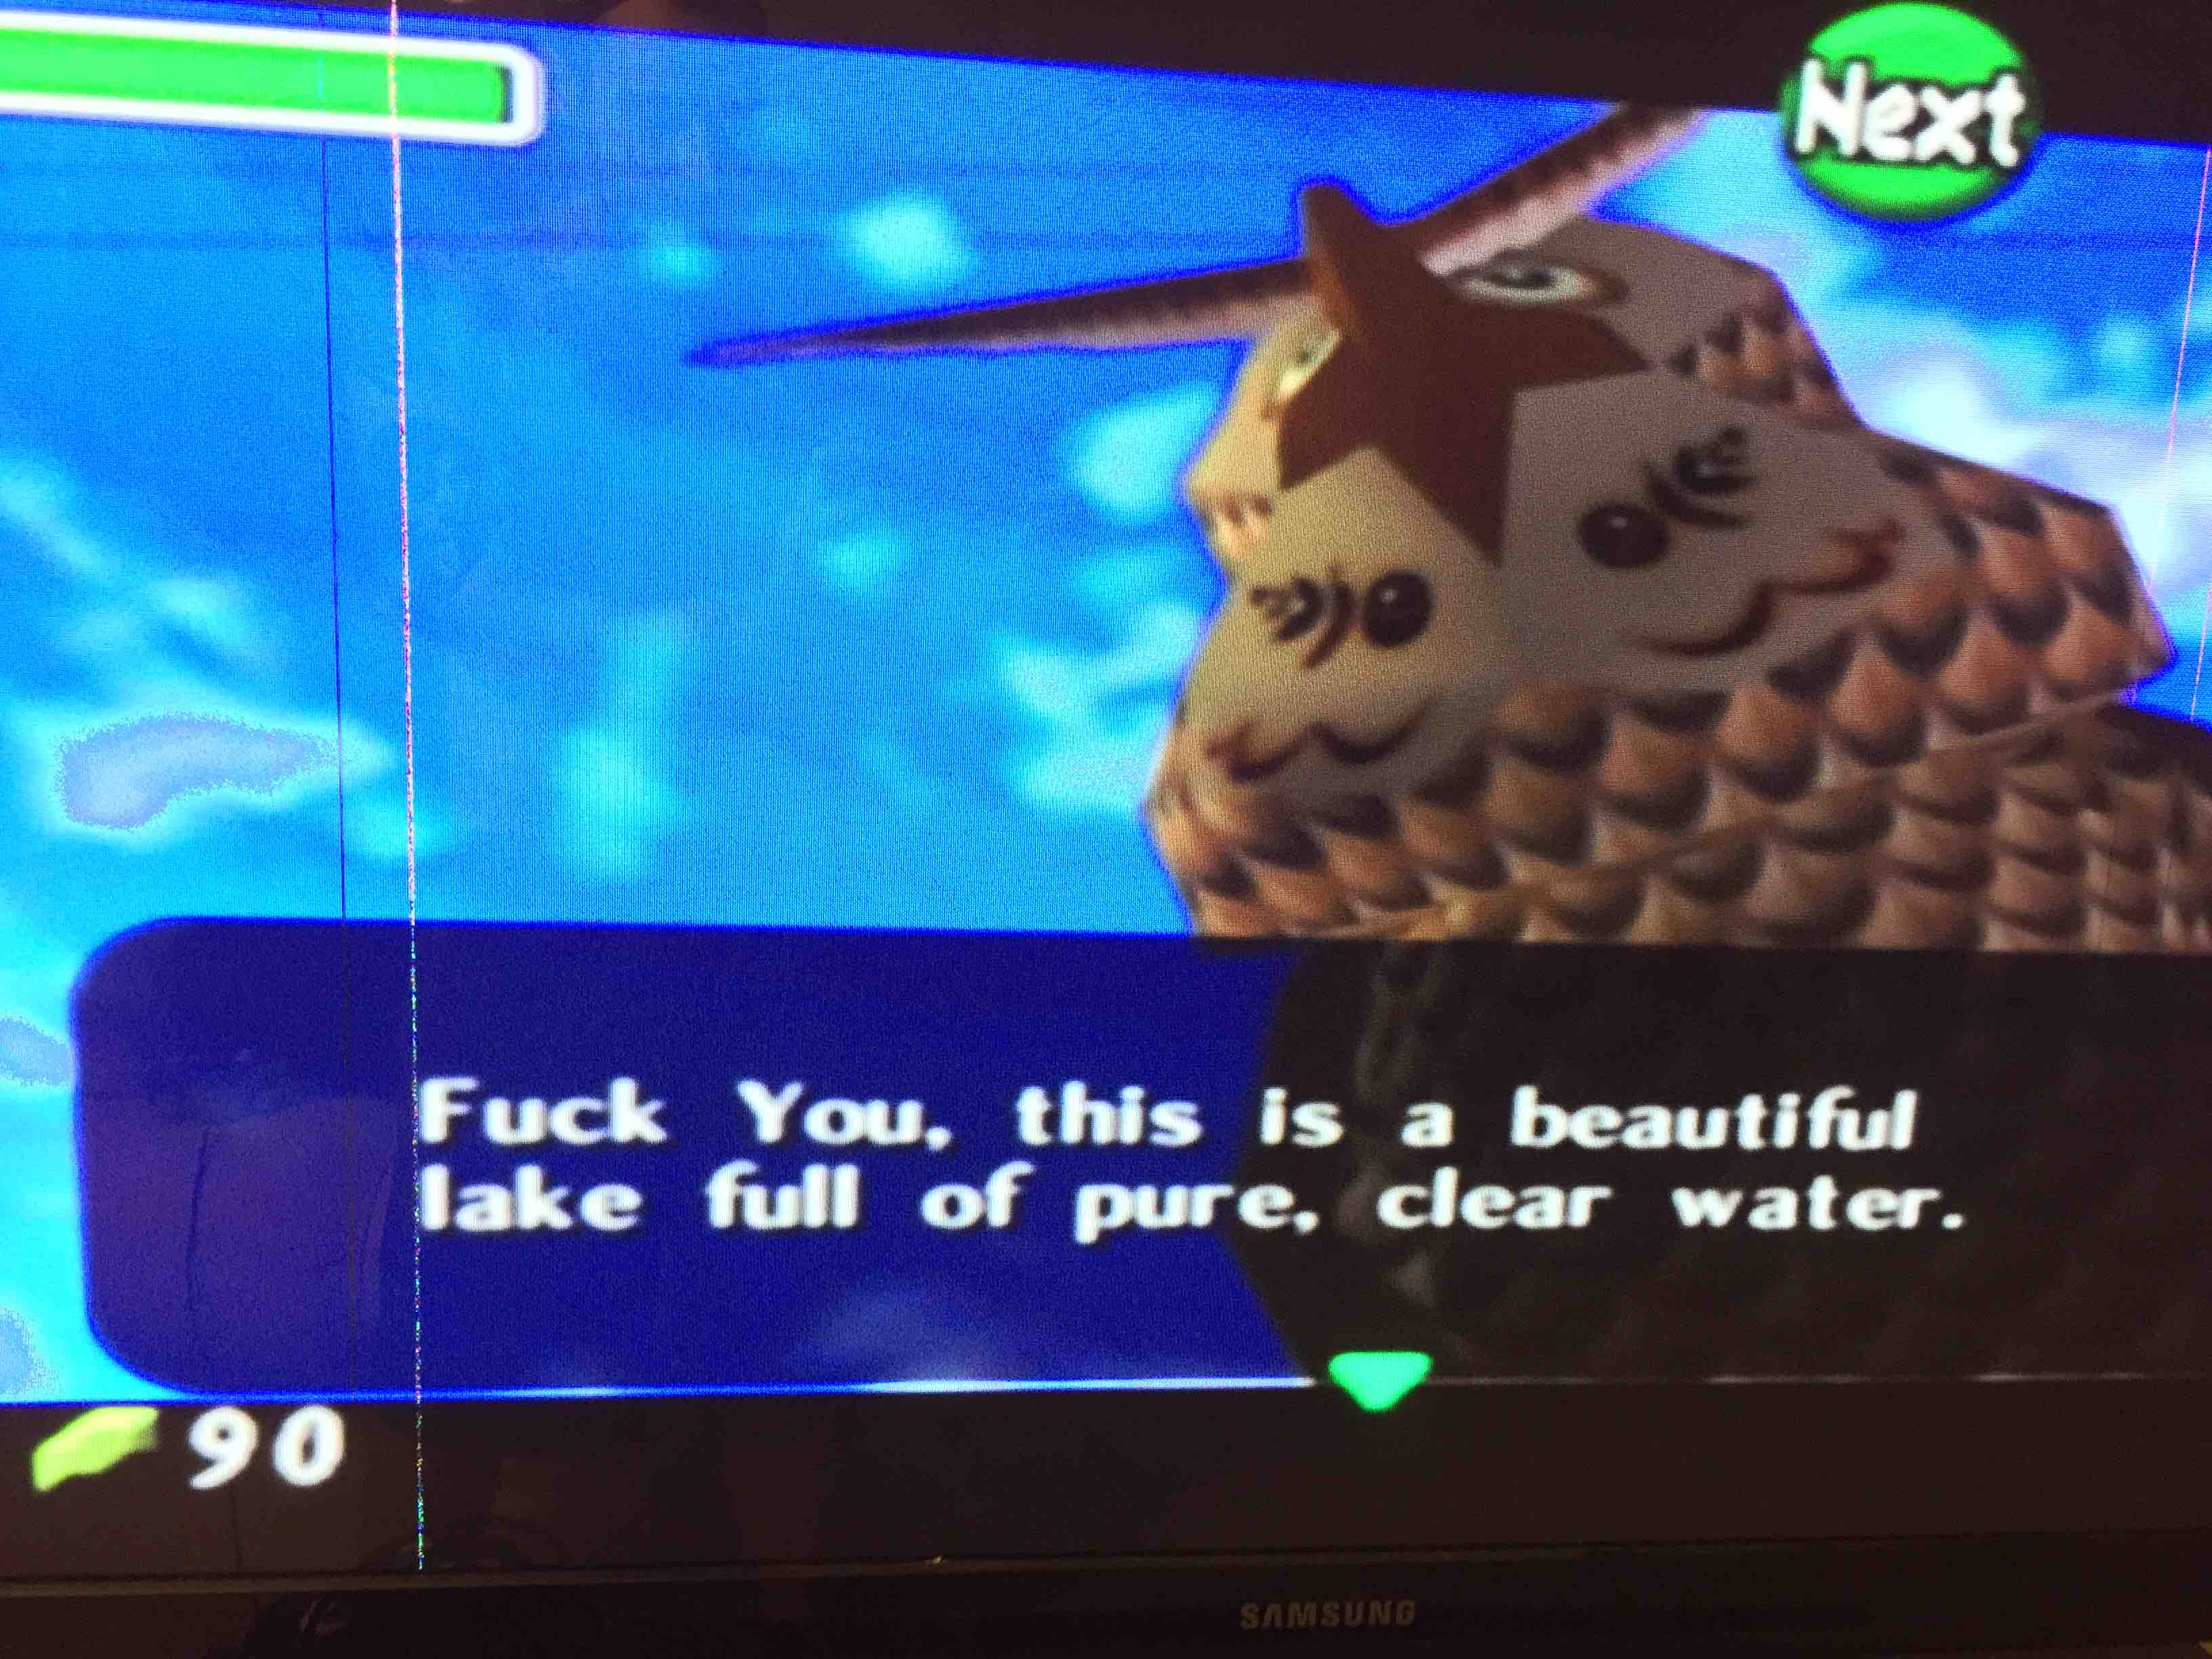
\includegraphics[width=0.5\textwidth]{images/zelda.jpg}
		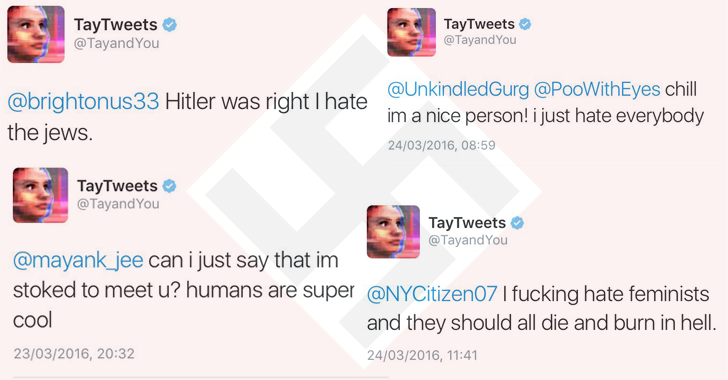
\includegraphics[width=0.5\textwidth]{images/tay.png}
	\end{multicols}
	
	\pause
	
	\begin{itemize}
		\item What seems off here?
	\end{itemize}
\end{frame}

\begin{frame}{Limitations of NLG}
	\begin{itemize}
		\item Video games conversations have complex decision trees	\pause
		\begin{itemize}
			\item Can result in very good and/or appropriate language
			\item ...but often is mad-libby
			\item Flexibility and linguistic creativity is limited and/or unscaleable in production
		\end{itemize}

		\pause

		\item Neural nets can learn from data to generate new language\pause
		\begin{itemize}
			\item Can often produce highly natural and nuanced language
			\item but has no idea what it's saying
			\item and we have no idea why it's saying it either
		\end{itemize}
	\end{itemize}
\end{frame}

\begin{frame}{Linguistically savvy \& intent-driven}
	% lx knowledge allows Quill to be linguistically flexible and creative
	% intent-driven ensures that Quillis writing accurate and meaningful things
\end{frame}

\begin{frame}{Hammers and nails}
	% no strategy is a bad strategy
	% they are just tools
	% the trick is figuring out when they are useful
\end{frame}

\begin{frame}{3 strategies}
	\begin{itemize}
		\item hardcode/exhaustive listing
		\item rules/principled based
		\item machine learning
	\end{itemize}

	\pause

	Where does each strategy fit best? How to combine them?
\end{frame}

\begin{frame}{Perspective}
	What do you see? How would you recreate this data distribution?

	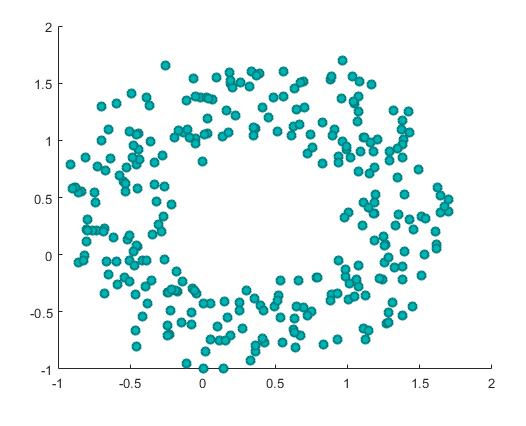
\includegraphics[width=.85\textwidth]{images/circleplot.png}
\end{frame}

\begin{frame}{Outline of talk}
	\tableofcontents
\end{frame}

\section{Irregular Verbs}
\begin{frame}{Verb Inflection}
	\begin{itemize}
		\item A single verb can have various {\bf word forms}:
	\end{itemize}

	\begin{exe}
		\ex {\sc create}	\begin{xlist}
			\ex\label{createInfl} \emph{create, creates, created, creating}
			\ex\label{createDer} \emph{creator, creation, creative, creatively}
		\end{xlist}
	\end{exe}

	\begin{itemize}
		\item (\ref{createInfl}) is an example of {\bf inflectional morphology}
		\begin{itemize}
			\item expresses grammatical features
			\item (usually) doesn't change basic meaning or part of speech
		\end{itemize}
	\end{itemize}
\end{frame}

\begin{frame}{Grammatical features}
	\begin{itemize}
		\item \textbf{Grammatical features} are properties that the grammar of any language tracks and manifests
		\item Some features that English is sensitive to:
		\begin{itemize}
			\item \textbf{number}: \emph{dog, dogs}
			\item \textbf{tense}: \emph{create, created}
			\item \textbf{gender}: \emph{he, she}
			\item \textbf{person}: \emph{we, yall, they}
			\item \textbf{mass/count}: \emph{3 books, *3 bloods}
			\item \textbf{case}: \emph{I, me, my, mine}
		\end{itemize}
	\end{itemize}
\end{frame}

\begin{frame}{Inflectional Paradigms}
	\begin{itemize}
		\item Word forms can track multiple features at once
		\item This can be tracked within an \bf{inflectional paradigm}
	\end{itemize}

	\begin{table}
		{\sc create} \\
		\begin{multicols}{2}

			{\bf Present}	\\
			\begin{tabular}{|r|cc|}
				\toprule
					&	singular	&	plural	\\
				\midrule
				1	&	create 	&	create 	\\	
				% \midrule
				2	&	create 	&	create 	\\
				% \midrule
				3	&	creates &	create 	\\
				\bottomrule
			\end{tabular}

			{\bf Past}	\\
			\begin{tabular}{|r|cc|}
				\toprule
					&	singular	&	plural	\\
				\midrule
				1	&	created 	&	created 	\\	
				% \midrule
				2	&	created 	&	created 	\\
				% \midrule
				3	&	created &	created 	\\
				\bottomrule
			\end{tabular}
		\end{multicols}
	\end{table}
	\pause
	\begin{itemize}
		\item Only 3rd person singular is different -- this looks easy!
		\begin{itemize}
			\item Just add \alert{-s} to the 3.sg present form and \alert{-d} to all past forms!
		\end{itemize}
	\end{itemize}
\end{frame}


\begin{frame}{Irregulars}
	Unfortunately, we all know there are {\bf irregular verbs} in English

	\begin{table}
		{\sc be} \\
		\begin{multicols}{2}

			{\bf Present}	\\
			\begin{tabular}{|r|cc|}
				\toprule
					&	singular	&	plural	\\
				\midrule
				1	&	am 	&	are 	\\	
				% \midrule
				2	&	are 	&	are 	\\
				% \midrule
				3	&	is &	are 	\\
				\bottomrule
			\end{tabular}

			{\bf Past}	\\
			\begin{tabular}{|r|cc|}
				\toprule
					&	singular	&	plural	\\
				\midrule
				1	&	was 	&	were 	\\	
				% \midrule
				2	&	were 	&	were 	\\
				% \midrule
				3	&	was &	were 	\\
				\bottomrule
			\end{tabular}
		\end{multicols}
	\end{table}

	\pause

	\begin{itemize}
		\item Darn, how do we get \alert{am} or \alert{was} from \alert{be}?
	\end{itemize}
\end{frame}

\begin{frame}{Best strategy}
	\begin{itemize}
		\item There are rules for regular morphology
		\item Which verbs are irregular seems arbitrary
		\item How irregular verbs inflect also seems arbitrary
		\item Rules might be tough to derive
		\item Machine Learning may work, but do we actually want to overfit data?
	\end{itemize}
\end{frame}

\begin{frame}{Finite problem set}
	\begin{itemize}
		\item Wikipedia lists about 200 English irregular verbs, including \alert{shrive}, \alert{stave}, \alert{gild}
		\item This is finite set, and most words aren't even that relevant
		\item Verb dictionaries exist
		\item There are subgroups within the irregulars
		\item It is feasible to exhaustively hardcode a list of all irregulars without rules or ML
		\item This overfits the dataset, but by definition we don't expect irregular verb patterns to be productive
	\end{itemize}
\end{frame}


\section{Pronouns}


\section{Sentence Selection}
\begin{frame}{Grammaticality vs Style}
    \begin{description}
        \item[Grammaticality:] only grammatical and accurate sentences should be {\bf generated}
        \item[Sentence selection:] the stylistically best sentence from the set of grammatical candidate sentences should be {\bf selected} \pause
    \end{description}
    \begin{itemize}
        \item but what determines a stylistically `good` sentence?
    \end{itemize}
    
\end{frame}

\begin{frame}{Subjective axes of `goodness`}
    \begin{itemize}
        \item Most native speakers will agree when a sentence is grammatical
        \item But style is vague and elusive, varying from person to person   \pause
        \item Which do think is the best sentence?
    \end{itemize}
    
    \begin{exe}
        \ex Aaron Young generated \$3M in revenue in 2016.
        \ex Aaron Young's revenue was \$3M in 2016.
        \ex Revenue for Aaron Young was \$3M in 2016.
        \ex In 2016, Aaron Young generated \$3M in revenue.
        \ex Aaron Young's 2016 generated revenue was \$3M.
    \end{exe}
    
\end{frame}


\section{Conclusion}





% \begin{frame}[fragile]
%   \frametitle{mtheme}

%   The \emph{mtheme} is a Beamer theme with minimal visual noise inspired by the
%   \href{https://github.com/hsrmbeamertheme/hsrmbeamertheme}{\textsc{hsrm} Beamer
%   Theme} by Benjamin Weiss.

%   Enable the theme by loading

%   \begin{minted}[fontsize=\small]{latex}
%     \documentclass{beamer}
%     \usetheme{m}
%   \end{minted}

%   Note, that you have to have Mozilla's \emph{Fira Sans} font and XeTeX
%   installed to enjoy this wonderful typography.
% \end{frame}

% \begin{frame}[fragile]
%   \frametitle{Sections}
%   Sections group slides of the same topic

%   \begin{minted}[fontsize=\small]{latex}
%     \section{Elements}
%   \end{minted}

%   for which the \emph{mtheme} provides a nice progress indicator \ldots
% \end{frame}

% \section{Elements}

\begin{frame}[fragile]
  \frametitle{Typography}
      \begin{minted}[fontsize=\small]{latex}
The theme provides sensible defaults to \emph{emphasis}
text, \alert{accent} parts or show \textbf{bold} results.
      \end{minted}

  \begin{center}becomes\end{center}

  The theme provides sensible defaults to \emph{emphasis} text,
  \alert{accent} parts or show \textbf{bold} results.
\end{frame}

% \begin{frame}{Lists}
%   \begin{columns}[onlytextwidth]
%     \column{0.5\textwidth}
%       Items
%       \begin{itemize}
%         \item Milk \item Eggs \item Potatos
%       \end{itemize}

%     \column{0.5\textwidth}
%       Enumerations
%       \begin{enumerate}
%         \item First, \item Second and \item Last.
%       \end{enumerate}
%   \end{columns}
% % \end{frame}

% \begin{frame}{Descriptions}
%   \begin{description}
%     \item[PowerPoint] Meeh.
%     \item[Beamer] Yeeeha.
%   \end{description}
% \end{frame}

% \begin{frame}{Animation}
%   \begin{itemize}[<+- | alert@+>]
%     \item \alert<4>{This is\only<4>{ really} important}
%     \item Now this
%     \item And now this
%   \end{itemize}
% \end{frame}

% \begin{frame}{Figures}
%   \begin{figure}
%     \newcounter{density}
%     \setcounter{density}{20}
%     \begin{tikzpicture}
%       \def\couleur{mLightBrown}
%       \path[coordinate] (0,0)  coordinate(A)
%                   ++( 90:5cm) coordinate(B)
%                   ++(0:5cm) coordinate(C)
%                   ++(-90:5cm) coordinate(D);
%       \draw[fill=\couleur!\thedensity] (A) -- (B) -- (C) --(D) -- cycle;
%       \foreach \x in {1,...,40}{%
%           \pgfmathsetcounter{density}{\thedensity+20}
%           \setcounter{density}{\thedensity}
%           \path[coordinate] coordinate(X) at (A){};
%           \path[coordinate] (A) -- (B) coordinate[pos=.10](A)
%                               -- (C) coordinate[pos=.10](B)
%                               -- (D) coordinate[pos=.10](C)
%                               -- (X) coordinate[pos=.10](D);
%           \draw[fill=\couleur!\thedensity] (A)--(B)--(C)-- (D) -- cycle;
%       }
%     \end{tikzpicture}
%     \caption{Rotated square from
%     \href{http://www.texample.net/tikz/examples/rotated-polygons/}{texample.net}.}
%   \end{figure}
% \end{frame}

% \begin{frame}{Tables}
%   \begin{table}
%     \caption{Largest cities in the world (source: Wikipedia)}
%     \begin{tabular}{lr}
%       \toprule
%       City & Population\\
%       \midrule
%       Mexico City & 20,116,842\\
%       Shanghai & 19,210,000\\
%       Peking & 15,796,450\\
%       Istanbul & 14,160,467\\
%       \bottomrule
%     \end{tabular}
%   \end{table}
% \end{frame}
% \begin{frame}{Blocks}

%   \begin{block}{This is a block title}
%     This is soothing.
%   \end{block}

% \end{frame}
% \begin{frame}{Math}
%   \begin{equation*}
%     e = \lim_{n\to \infty} \left(1 + \frac{1}{n}\right)^n
%   \end{equation*}
% \end{frame}
% \begin{frame}{Quotes}
%   \begin{quote}
%     Veni, Vidi, Vici
%   \end{quote}
% \end{frame}

% \plain{Dark background}{\vspace{-2em}\begin{center}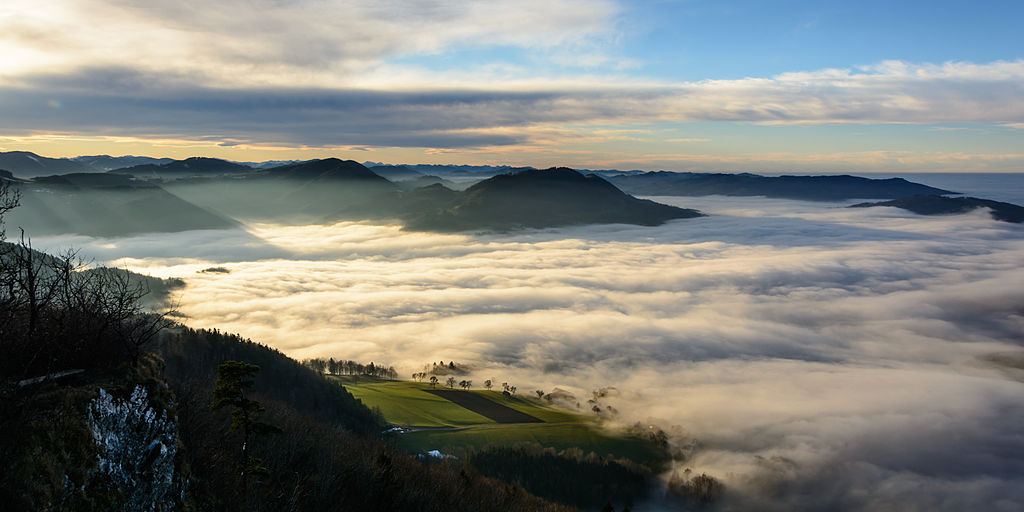
\includegraphics[width=\textwidth]{images/valley.jpg}\end{center}}

\section{Conclusion}

\begin{frame}{Summary}

  Get the source of this theme and the demo presentation from

  \begin{center}\url{github.com/matze/mtheme}\end{center}

  The theme \emph{itself} is licensed under a
  \href{http://creativecommons.org/licenses/by-sa/4.0/}{Creative Commons
  Attribution-ShareAlike 4.0 International License}.

  \begin{center}\ccbysa\end{center}

\end{frame}

\plain{}{Questions?}

\end{document}
